\documentclass[11pt, A4paper,norsk]{article}
\usepackage[utf8]{inputenc}
\usepackage[T1]{fontenc}
\usepackage{babel}
\usepackage{amsmath}
\usepackage{amsfonts}
\usepackage{amsthm}
\usepackage{amssymb}
\usepackage[colorlinks]{hyperref}
\usepackage{listings}
\usepackage{color}
\usepackage{hyperref}
\usepackage{graphicx}
\usepackage{cite}
\usepackage{textcomp}
\usepackage{float}

\definecolor{dkgreen}{rgb}{0,0.6,0}
\definecolor{gray}{rgb}{0.5,0.5,0.5}
\definecolor{daynineyellow}{rgb}{1.0,0.655,0.102}
\definecolor{url}{rgb}{0.1,0.1,0.4}

\lstset{frame=tb,
	language=Python,
	aboveskip=3mm,
	belowskip=3mm,
	showstringspaces=false,
	columns=flexible,
	basicstyle={\small\ttfamily},
	numbers=none,
	numberstyle=\tiny\color{gray},
	keywordstyle=\color{blue},
	commentstyle=\color{daynineyellow},
	stringstyle=\color{dkgreen},
	breaklines=true,
	breakatwhitespace=true,
	tabsize=3
}

\lstset{inputpath="C:/Users/Torstein/Documents/UiO/Fys2140/Python programmer"}
\graphicspath{{C:/Users/Torstein/Documents/UiO/Fys2140/"Python programmer"/}}
\hypersetup{colorlinks, urlcolor=url}

\author{Torstein Solheim Ølberg}
\title{Svar på Oblig nr. 6 i Fys2140}



%\lstinputlisting{Filnavn! type kodefil}
%\includegraphics[width=12.6cm,height=8cm]{Filnavn! type png}



\begin{document}
\maketitle
	\begin{center}
\Large \textbf{Oppgaver}
	\end{center}








\clearpage
		\paragraph{1.}
			\subparagraph{a)}
				\begin{gather*}
\psi_0(x) = \left( \frac{m \omega}{\pi \hbar} \right)^{\frac{1}{4}} e^{- \frac{m \omega}{2 \hbar} x^2} \\
\psi_2 = A_2 (a_+)^2 \psi_0(x) = A_2 \left( \frac{1}{\sqrt{2 \hbar m \omega}} \left( - \hbar \frac{d}{dx} + m \omega x \right) \right)^2 \left( \frac{m \omega}{\pi \hbar} \right)^{\frac{1}{4}} e^{- \frac{m \omega}{2 \hbar} x^2} \\
\psi_2 = \frac{A_2}{2 \hbar m \omega} \left( \frac{m \omega}{\pi \hbar} \right)^{\frac{1}{4}} \left( \hbar^2 \frac{d^2}{dx^2} - \hbar \frac{d}{dx} x m \omega - x m \omega \hbar \frac{d}{dx} + m^2 \omega^2 x^2 \right) e^{-\frac{m \omega}{2 \hbar} x^2} \\
\frac{d}{dx} e^{- \frac{m \omega}{2 \hbar} x^2} = - \frac{m \omega}{\hbar} x e^{- \frac{m \omega}{2 \hbar} x^2} \\
\frac{d}{dx} x e^{- \frac{m \omega}{2 \hbar} x^2} = e^{- \frac{m \omega}{2 \hbar} x^2} + - \frac{m \omega}{\hbar} x^2 e^{- \frac{m \omega}{2 \hbar} x^2} = e^{- \frac{m \omega}{2 \hbar} x^2} \left( 1 - \frac{m \omega}{\hbar} x^2 \right) \\
\frac{d^2}{dx^2} e^{- \frac{m \omega}{2 \hbar} x^2} = - \frac{m \omega}{\hbar} \left( e^{- \frac{m \omega}{2 \hbar} x^2} + - \frac{m \omega}{\hbar} x^2 e^{- \frac{m \omega}{2 \hbar} x^2} \right) = - \frac{m \omega}{\hbar} e^{- \frac{m \omega}{2 \hbar} x^2} \left( 1 - \frac{m \omega}{\hbar} x^2 \right) \\
- \hbar^2 \frac{m \omega}{\hbar} e^{- \frac{m \omega}{2 \hbar} x^2} \left( 1 - \frac{m \omega}{\hbar} x^2 \right) - \hbar e^{- \frac{m \omega}{2 \hbar} x^2} \left( 1 - \frac{m \omega}{\hbar} x^2 \right) m \omega + m \omega \hbar \frac{m \omega}{\hbar} x^2 e^{- \frac{m \omega}{2 \hbar} x^2} + m^2 \omega^2 x^2 e^{-\frac{m \omega}{2 \hbar} x^2} \\
- \hbar m \omega e^{-\frac{m \omega}{2 \hbar} x^2} + m^2 \omega^2 x^2 e^{-\frac{m \omega}{2 \hbar} x^2} - \hbar m \omega e^{-\frac{m \omega}{2 \hbar} x^2} + m^2 \omega^2 x^2 e^{-\frac{m \omega}{2 \hbar} x^2} + m^2 \omega^2 x^2 e^{-\frac{m \omega}{2 \hbar} x^2} + m^2 \omega^2 x^2 e^{-\frac{m \omega}{2 \hbar} x^2} \\
- 2 \hbar m \omega e^{-\frac{m \omega}{2 \hbar} x^2} + 4 m^2 \omega^2 x^2 e^{-\frac{m \omega}{2 \hbar} x^2} \\
\psi_2 = \frac{A_2}{2 \hbar m \omega}  e^{- \frac{m \omega}{2 \hbar} x^2} \left( \frac{m \omega}{\pi \hbar} \right)^{\frac{1}{4}} \left( - 2 \hbar m \omega + 4 m^2 \omega^2 x^2 \right) \\
\psi_2 = A_2  e^{- \frac{m \omega}{2 \hbar} x^2} \left( \frac{m \omega}{\pi \hbar} \right)^{\frac{1}{4}} \left( \frac{2 m \omega x^2}{\hbar} - 1 \right) \\
\psi_2 = \sqrt{2} e^{- \frac{m \omega}{2 \hbar} x^2} \left( \frac{m \omega}{\pi \hbar} \right)^{\frac{1}{4}} \left( \frac{2 m \omega x^2}{\hbar} - 1 \right) \\
\text{Fikk normaliseringen fra den generelle formelen for $A$, $A_n = \frac{1}{\sqrt{n!}}$}
				\end{gather*}









			\subparagraph{b)} \text{ }
				\begin{figure}[H]
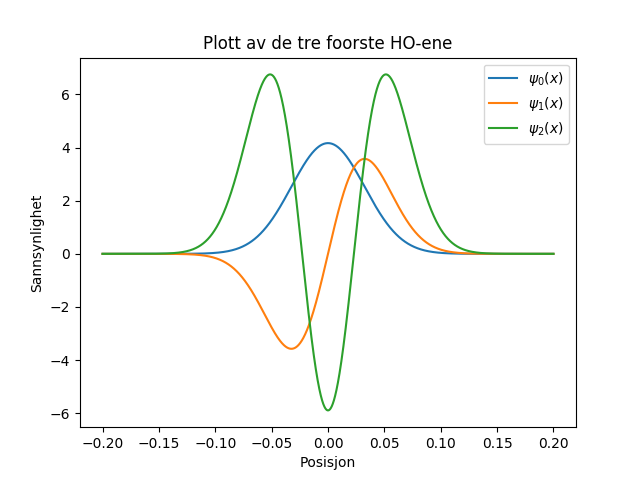
\includegraphics[width=12.6cm,height=9cm]{Figur_04.png}
				\end{figure}
\lstinputlisting{Oblig6_1b.py}









			\subparagraph{c)}
				\begin{gather*}
\int_{- \infty}^{\infty} \psi_0(x)^{*} \psi_1(x) dx = 0 \\
\int_{- \infty}^{\infty} \left( \frac{m \omega}{\pi \hbar} \right)^{\frac{1}{4}} e^{- \frac{m \omega}{2 \hbar} x^2} \cdot \left( \frac{m \omega}{\pi \hbar} \right)^{\frac{1}{4}} \sqrt{\frac{2 m \omega}{\hbar}} x e^{- \frac{m \omega}{2 \hbar} x^2} dx = 0 \\
\frac{m \omega}{\hbar} \sqrt{\frac{2}{\pi}} \int_{- \infty}^{\infty} x e^{- \frac{m \omega}{\hbar} x^2} dx = 0 \\
\frac{m \omega}{\hbar} \sqrt{\frac{2}{\pi}} \cdot 0 = 0 \\
\int_{- \infty}^{\infty} \psi_1(x)^{*} \psi_2(x) dx = 0 \\
\int_{- \infty}^{\infty} \left( \frac{m \omega}{\pi \hbar} \right)^{\frac{1}{4}} \sqrt{\frac{2 m \omega}{\hbar}} e^{- \frac{m \omega}{2 \hbar} x^2} \cdot \sqrt{2} e^{- \frac{m \omega}{2 \hbar} x^2} \left( \frac{m \omega}{\pi \hbar} \right)^{\frac{1}{4}} \left( \frac{2 m \omega x^2}{\hbar} - 1 \right) dx = 0 \\
\frac{2}{\sqrt{\pi}} \left( \frac{2 m \omega}{\hbar} \int_{- \infty}^{\infty} x^2 e^{- \frac{m \omega}{\hbar} x^2} - \int_{- \infty}^{\infty} e^{- \frac{m \omega}{\hbar} x^2} \right) dx = 0 \\
\frac{2}{\sqrt{\pi}} \left( \frac{2 m \omega}{\hbar} \sqrt{\frac{\pi}{2^2 \left( \frac{m \omega}{\hbar} \right)^{3}}} - \sqrt{\frac{\pi}{\frac{m \omega}{\hbar}}} \right) = 0 \\
\frac{2}{\sqrt{\pi}} \left( \sqrt{\frac{\pi}{\frac{m \omega}{\hbar}}} - \sqrt{\frac{\pi}{\frac{m \omega}{\hbar}}} \right) = 0 \\
\frac{2}{\sqrt{\pi}} \cdot 0 = 0 \\
\int_{- \infty}^{\infty} \psi_0^{*}(x) \psi_2(x) dx = 0 \\
\int_{- \infty}^{\infty} \left( \frac{m \omega}{\pi \hbar} \right)^{\frac{1}{4}} e^{- \frac{m \omega}{2 \hbar} x^2} \cdot \sqrt{2} e^{- \frac{m \omega}{2 \hbar} x^2} \left( \frac{m \omega}{\pi \hbar} \right)^{\frac{1}{4}} \left( \frac{2 m \omega x^2}{\hbar} - 1 \right) dx = 0 \\
\sqrt{2} \left( \frac{m \omega}{\pi \hbar} \right)^{\frac{1}{2}} \left( \frac{2 m \omega}{\hbar} \int_{- \infty}^{\infty} x^2 e^{- \frac{m \omega}{\hbar} x^2} - \int_{- \infty}^{\infty} e^{- \frac{m \omega}{\hbar} x^2} \right) dx = 0 \\
\sqrt{2} \left( \frac{m \omega}{\pi \hbar} \right)^{\frac{1}{2}} \left( \sqrt{\frac{\pi}{\frac{m \omega}{\hbar}}} - \sqrt{\frac{\pi}{\frac{m \omega}{\hbar}}} \right) = 0 \\
\sqrt{2} \left( \frac{m \omega}{\pi \hbar} \right)^{\frac{1}{2}} \cdot 0 = 0
				\end{gather*}
			








		\paragraph{2.}
			\subparagraph{a)}
				\begin{flushleft}
Begynner med å regne ut forventningsverdier for $\psi_0$.
				\end{flushleft}
				\begin{gather*}
\text{Det er enkelt å se at $\psi_0$ er symetrisk om y-aksen, og det er derfor} \\
\text{lett å skjønne at forventningsverdien til $x$ for $\psi_0$ er $0$}
				\end{gather*}
				\begin{gather*}
\langle x^2 \rangle = \int_{- \infty}^{\infty} \psi_0^{*} x^2 \psi_0 dx \\
\int_{- \infty}^{\infty} \left( \frac{m \omega}{\pi \hbar} \right)^{\frac{1}{4}} e^{- \frac{m \omega}{2 \hbar} x^2} x^2 \left( \frac{m \omega}{\pi \hbar} \right)^{\frac{1}{4}} e^{- \frac{m \omega}{2 \hbar} x^2} dx \\
\left( \frac{m \omega}{\pi \hbar} \right)^{\frac{1}{2}} \int_{- \infty}^{\infty} x^2 e^{- \frac{m \omega}{\hbar} x^2} dx \\
\left( \frac{m \omega}{\pi \hbar} \right)^{\frac{1}{2}} \sqrt{\frac{\pi}{2^2 \left( \frac{m \omega}{\hbar} \right)^{3}}} = \left( \frac{m \omega}{\pi \hbar} \right)^{\frac{1}{2}} \left( \frac{\pi \hbar^3}{4 m^3 \omega^3} \right)^{\frac{1}{2}} = \left( \frac{\hbar^2}{4 m^2 \omega^2} \right)^{\frac{1}{2}} = \frac{\hbar}{2 m \omega} \\
\langle x^2 \rangle = \frac{\hbar}{2 m \omega}
				\end{gather*}
				\begin{gather*}
\text{Det er like sannsynlig at en partikkel har en bevegelsesmengde i en hvilken som} \\
\text{helst retning, og forventningsverdien til $p$ blir da $0$. Dette kan også lett sees ved} \\
\text{likningen under og at vi fra utregningene over, vet at $\langle x \rangle$ er tidsuavhengig.} \\
\langle p \rangle = m \frac{d}{dt} \langle x \rangle = 0 \\
\langle p \rangle = - i \hbar \int_{- \infty}^{\infty} \psi_0^{*} \frac{d}{dx} \psi_0 dx \\
- i \hbar \left( \frac{m \omega}{\pi \hbar} \right)^{\frac{1}{2}} \int_{- \infty}^{\infty} e^{- \frac{m \omega}{2 \hbar} x^2} \frac{d}{dx} e^{- \frac{m \omega}{2 \hbar} x^2} dx \\
i \hbar \left( \frac{m \omega}{\pi \hbar} \right)^{\frac{1}{2}} \frac{m \omega}{\hbar} \int_{- \infty}^{\infty} x e^{- \frac{m \omega}{\hbar} x^2} dx \\
				\end{gather*}
				\begin{gather*}
\langle p^2 \rangle = \int_{- \infty}^{\infty} \psi_0^{*} i^2 \hbar^2 \frac{d^2}{dx^2} \psi_0 dx \\
- \hbar^2 \int_{- \infty}^{\infty} \left( \frac{m \omega}{\pi \hbar} \right)^{\frac{1}{4}} e^{- \frac{m \omega}{2 \hbar} x^2} \frac{d^2}{dx^2} \left( \frac{m \omega}{\pi \hbar} \right)^{\frac{1}{4}} e^{- \frac{m \omega}{2 \hbar} x^2} dx \\
\hbar^2 \int_{- \infty}^{\infty} \left( \frac{m \omega}{\pi \hbar} \right)^{\frac{1}{4}} e^{- \frac{m \omega}{2 \hbar} x^2} \left( \frac{m \omega}{\pi \hbar} \right)^{\frac{1}{4}} \frac{m \omega}{\hbar} e^{- \frac{m \omega}{2 \hbar} x^2} \left( 1 - \frac{m \omega}{\hbar} x^2 \right) dx \\
\hbar^2 \left( \frac{m \omega}{\pi \hbar} \right)^{\frac{1}{2}} \frac{m \omega}{\hbar} \left( \int_{- \infty}^{\infty} e^{- \frac{m \omega}{\hbar} x^2} - \frac{m \omega}{\hbar} \int_{- \infty}^{\infty} x^2 e^{- \frac{m \omega}{2 \hbar} x^2} \right) \\
\hbar^2 \left( \frac{m \omega}{\pi \hbar} \right)^{\frac{1}{2}} \frac{m \omega}{\hbar} \left( \sqrt{\frac{\pi}{\frac{m \omega}{\hbar}}} - \frac{m \omega}{\hbar} \sqrt{\frac{\pi}{2^2 \left( \frac{m \omega}{\hbar} \right)^{3}}} \right) \\
\hbar^2 \left( \frac{m \omega}{\pi \hbar} \right)^{\frac{1}{2}} \frac{m \omega}{\hbar} \left( \sqrt{\frac{\pi}{\frac{m \omega}{\hbar}}} - \frac{1}{2} \sqrt{\frac{\pi}{\frac{m \omega}{\hbar}}} \right) \\
\langle p^2 \rangle = \frac{\hbar m \omega}{2}
				\end{gather*}
				\begin{flushleft}
Fortsetter deretter med forventningsverdiene for $\psi_1$.
				\end{flushleft}
				\begin{gather*}
\langle x \rangle = \int_{- \infty}^{\infty} \psi_1^{*} x \psi_1 dx \\
\int_{- \infty}^{\infty} \left( \frac{m \omega}{\pi \hbar} \right)^{\frac{1}{4}} \sqrt{\frac{2 m \omega}{\hbar}} x e^{- \frac{m \omega}{2 \hbar} x^2} x \left( \frac{m \omega}{\pi \hbar} \right)^{\frac{1}{4}} \sqrt{\frac{2 m \omega}{\hbar}} x e^{- \frac{m \omega}{2 \hbar} x^2} \\
\left( \frac{m \omega}{\pi \hbar} \right)^{\frac{1}{2}} \frac{2 m \omega}{\hbar} \int_{- \infty}^{\infty} x^3 e^{- \frac{m \omega}{\hbar} x^2} dx \\
\int_{- \infty}^{\infty} x^3 e^{- \frac{m \omega}{\hbar} x^2} dx = 0 \\
\langle x \rangle = 0
				\end{gather*}
				\begin{gather*}
\langle x^2 \rangle = \int_{- \infty}^{\infty} \psi_1^{*} x^2 \psi_1 dx \\
\int_{- \infty}^{\infty} \left( \frac{m \omega}{\pi \hbar} \right)^{\frac{1}{4}} \sqrt{\frac{2 m \omega}{\hbar}} x e^{- \frac{m \omega}{2 \hbar} x^2} x^2 \left( \frac{m \omega}{\pi \hbar} \right)^{\frac{1}{4}} \sqrt{\frac{2 m \omega}{\hbar}} x e^{- \frac{m \omega}{2 \hbar} x^2} \\
\left( \frac{m \omega}{\pi \hbar} \right)^{\frac{1}{2}} \frac{2 m \omega}{\hbar} \int_{- \infty}^{\infty} x^4 e^{- \frac{m \omega}{\hbar} x^2} dx \\
\int_{- \infty}^{\infty} x^4 e^{- \frac{m \omega}{\hbar} x^2} dx = 2 \int_{0}^{\infty} x^4 e^{- \frac{m \omega}{\hbar} x^2} dx = \left( \frac{m \omega}{\hbar} \right)^{- \frac{5}{2}} \Gamma\left( \frac{5}{2} \right) = \left( \frac{m \omega}{\hbar} \right)^{- \frac{5}{2}} \frac{3}{4} \sqrt{\pi} \\
\left( \frac{m \omega}{\pi \hbar} \right)^{\frac{1}{2}} \frac{2 m \omega}{\hbar} \left( \frac{m \omega}{\hbar} \right)^{- \frac{5}{2}} \frac{3}{4} \sqrt{\pi} = \left( \frac{m \omega}{\hbar} \right)^{-2} \frac{m \omega}{\hbar} \frac{3}{2} = \frac{3 \hbar}{2 m \omega} \\
\langle x^2 \rangle = \frac{3\hbar}{2 m \omega}
				\end{gather*}
				\begin{gather*}
\text{Det er fortsatt like sannsynlig at en partikkel har en bevegelsesmengde i en hvilken} \\
\text{som helst retning, og forventningsverdien til $p$ blir da $0$.} \\
				\end{gather*}
				\begin{gather*}
\langle p^2 \rangle = \int_{- \infty}^{\infty} \psi_1^{*} i^2 \hbar^2 \frac{d^2}{dx^2} \psi_1 dx \\
- \hbar^2 \int_{- \infty}^{\infty} \left( \frac{m \omega}{\pi \hbar} \right)^{\frac{1}{4}} \sqrt{\frac{2 m \omega}{\hbar}} x e^{- \frac{m \omega}{2 \hbar} x^2} \frac{d^2}{dx^2} \left( \frac{m \omega}{\pi \hbar} \right)^{\frac{1}{4}} \sqrt{\frac{2 m \omega}{\hbar}} x e^{- \frac{m \omega}{2 \hbar} x^2} dx \\
- 2 \hbar^2 \left( \frac{m \omega}{\pi \hbar} \right)^{\frac{1}{2}} \frac{m \omega}{\hbar} \int_{- \infty}^{\infty} x e^{- \frac{m \omega}{2 \hbar} x^2} \frac{d^2}{dx^2} x e^{- \frac{m \omega}{2 \hbar} x^2} dx \\
\frac{d^2}{dx^2} x e^{- \frac{m \omega}{2 \hbar} x^2} = \frac{d}{dx}  e^{- \frac{m \omega}{2 \hbar} x^2} \left( 1 - \frac{m \omega}{\hbar} x^2 \right) = \left( \frac{d}{dx} e^{- \frac{m \omega}{2 \hbar} x^2} - \frac{m \omega}{\hbar} \frac{d}{dx} x^2 e^{- \frac{m \omega}{2 \hbar} x^2} \right) \\
- \frac{m \omega}{\hbar} x e^{- \frac{m \omega}{2 \hbar} x^2} - \frac{m \omega}{\hbar} \left( 2x e^{- \frac{m \omega}{2 \hbar} x^2} - \frac{m \omega}{\hbar} x^3 e^{- \frac{m \omega}{2 \hbar} x^2} \right) \\
- \left( \frac{m \omega}{\hbar} \right) x e^{- \frac{m \omega}{2 \hbar} x^2} - 2 \left( \frac{m \omega}{\hbar} \right) x e^{- \frac{m \omega}{2 \hbar} x^2} + \left( \frac{m \omega}{\hbar} \right)^{2} x^3 e^{- \frac{m \omega}{2 \hbar} x^2} \\
- 3 \left( \frac{m \omega}{\hbar} \right) x e^{- \frac{m \omega}{2 \hbar} x^2} + \left( \frac{m \omega}{\hbar} \right)^{2} x^3 e^{- \frac{m \omega}{2 \hbar} x^2} \\
\left( \frac{m \omega}{\hbar} \right) x e^{- \frac{m \omega}{2 \hbar} x^2} \left( \frac{m \omega}{\hbar} x^2 - 3 \right) \\
- 2 \hbar^2 \left( \frac{m \omega}{\pi \hbar} \right)^{\frac{1}{2}} \frac{m \omega}{\hbar} \int_{- \infty}^{\infty} x e^{- \frac{m \omega}{2 \hbar} x^2} \left( \frac{m \omega}{\hbar} \right) x e^{- \frac{m \omega}{2 \hbar} x^2} \left( \frac{m \omega}{\hbar} x^2 - 3 \right) dx \\
- 2 \hbar^2 \left( \frac{m \omega}{\pi \hbar} \right)^{\frac{1}{2}} \left( \frac{m \omega}{\hbar} \right)^{2} \left( \int_{- \infty}^{\infty} - 3 x^2 e^{- \frac{m \omega}{\hbar} x^2} + \frac{m \omega}{\hbar} \int_{- \infty}^{\infty} x^4 e^{- \frac{m \omega}{\hbar} x^2} dx \right) \\
- 2 \hbar^2 \left( \frac{m \omega}{\pi \hbar} \right)^{\frac{1}{2}} \left( \frac{m \omega}{\hbar} \right)^{2} \left( - 3 \sqrt{\frac{\pi}{2^2 \left( \frac{m \omega}{\hbar} \right)^{3}}} + \frac{m \omega}{\hbar} \left( \frac{m \omega}{\hbar} \right)^{- \frac{5}{2}} \frac{3}{4} \sqrt{\pi} \right) \\
- 2 \hbar^2 \left( \frac{m \omega}{\pi \hbar} \right)^{\frac{1}{2}} \left( \frac{m \omega}{\hbar} \right)^{2} \sqrt{\pi} 3 \left( - \frac{1}{2} \left( \frac{\hbar}{m \omega} \right)^{\frac{3}{2}} + \frac{1}{4} \left( \frac{\hbar}{m \omega} \right)^{\frac{3}{2}} \right) \\
2 \hbar^2 \left( \frac{m \omega}{\pi \hbar} \right)^{\frac{1}{2}} \left( \frac{m \omega}{\hbar} \right)^{2} \sqrt{\pi} 3 \frac{1}{4} \left( \frac{\hbar}{m \omega} \right)^{\frac{3}{2}} \\
\frac{3}{2} \hbar^2 \left( \frac{m \omega}{\hbar} \right)^{2} \frac{\hbar}{m \omega} \\
\langle p^2 \rangle = \frac{3 \hbar m \omega}{2}
				\end{gather*}












			\subparagraph{b)}
				\begin{gather*}
\text{Begynner med å sjekke for $\psi_0$} \\
\sigma_x = \langle x^2 \rangle - \langle x \rangle^2 \\
\sigma_x = \frac{\hbar}{2 m \omega} - 0^2 = \frac{\hbar}{2 m \omega} \\
\sigma_p = \langle p^2 \rangle - \langle p \rangle^2 \\
\sigma_x = \frac{\hbar m \omega}{2} - 0^2 = \frac{\hbar m \omega}{2} \\
\sigma_x \sigma_p = \sqrt{\frac{\hbar}{2 m \omega} \frac{\hbar m \omega}{2}} = \sqrt{\frac{\hbar^2}{2^2}} = \frac{\hbar}{2} \\
\text{Fortsetter med $\psi_1$} \\
\sigma_x = \langle x^2 \rangle - \langle x \rangle^2 \\
\sigma_x = \frac{3\hbar}{2 m \omega} - 0^2 = \frac{3 \hbar}{2 m \omega} \\
\sigma_p = \langle p^2 \rangle - \langle p \rangle^2 \\
\sigma_p = \frac{3 \hbar m \omega}{2} - 0^2 = \frac{3 \hbar m \omega}{2} \\
\sigma_x \sigma_p = \sqrt{\frac{3 \hbar}{2 m \omega} \frac{3 \hbar m \omega}{2}} = \sqrt{\frac{9 \hbar^2}{4}} \\
\frac{3 \hbar}{2} \geq \frac{\hbar}{2}
				\end{gather*}










			\subparagraph{c)}
				\begin{gather*}
\text{Starter med $\psi_0$} \\
\langle K \rangle = \frac{1}{2} \frac{\langle p^2 \rangle}{m} = \frac{1}{2} \frac{\hbar m \omega}{2} \frac{1}{m} = \frac{\hbar \omega}{4} \\
\langle V \rangle = \frac{1}{2} m \omega^2 \langle x^2 \rangle = \frac{1}{2} m \omega^2 \frac{\hbar}{2 m \omega} = \frac{\hbar \omega}{4} \\
\langle E \rangle = \langle K \rangle + \langle V \rangle = \frac{\hbar \omega}{2} \\
\text{Fortsetter med $\psi_1$} \\
\langle K \rangle = \frac{1}{2} \frac{\langle p^2 \rangle}{m} = \frac{1}{2} \frac{3 \hbar m \omega}{2} \frac{1}{m} = \frac{3 \hbar \omega}{4} \\
\langle V \rangle = \frac{1}{2} m \omega^2 \langle x^2 \rangle = \frac{1}{2} m \omega^2 \frac{3\hbar}{2 m \omega} = \frac{3 \hbar \omega}{4} \\
\langle E \rangle = \langle K \rangle + \langle V \rangle = \frac{3 \hbar \omega}{2} \\
\text{Den totale energien $E$ er naturlig at er det dobbelte av den kinetiske} \\
\text{eller den potensielle energien fordi harmoniske svigninger veksler mellom å} \\
\text{ha bare potensiell og bare kinetisk energi}
				\end{gather*}
\end{document}